\documentclass[a4paper,12pt]{article} % тип документа

% Поля страниц
\usepackage[left=2.5cm,right=2.5cm,
    top=2cm,bottom=2cm,bindingoffset=0cm]{geometry}
    
%Пакет дял таблиц   
\usepackage{multirow}
\usepackage{longtable}
    
%Отступ после заголовка    
\usepackage{indentfirst}


% Рисунки
\usepackage{floatrow,graphicx,calc}
\usepackage{wrapfig}

% Создаёем новый разделитель
\DeclareFloatSeparators{mysep}{\hspace{1cm}}

% Ссылки?
\usepackage{hyperref}
\usepackage[rgb]{xcolor}
\hypersetup{				% Гиперссылки
    colorlinks=true,       	% false: ссылки в рамках
	urlcolor=blue          % на URL
}


%  Русский язык
\usepackage[T2A]{fontenc}			% кодировка
\usepackage[utf8]{inputenc}			% кодировка исходного текста
\usepackage[english,russian]{babel}	% локализация и переносы


% Математика
\usepackage{amsmath,amsfonts,amssymb,amsthm,mathtools, mathrsfs}


% Что-то 
\usepackage{wasysym}


\begin{document}
\begin{center}
	\footnotesize{ФЕДЕРАЛЬНОЕ ГОСУДАРСТВЕННОЕ АВТОНОМНОЕ ОБРАЗОВАТЕЛЬНОЕ 			УЧРЕЖДЕНИЕ ВЫСШЕГО ОБРАЗОВАНИЯ}\\
	\footnotesize{МОСКОВСКИЙ ФИЗИКО-ТЕХНИЧЕСКИЙ ИНСТИТУТ\\(НАЦИОНАЛЬНЫЙ 			ИССЛЕДОВАТЕЛЬСКИЙ УНИВЕРСИТЕТ)}\\
	\footnotesize{ФАКУЛЬТЕТ ОБЩЕЙ И ПРИКЛАДНОЙ ФИЗИКИ\\}
	\hfill \break
	\hfill\break
	\hfill\break
	\hfill \break
	\hfill \break
	\hfill \break
	\hfill \break
	\hfill \break
	\hfill \break
	\hfill \break
	\hfill \break
	\hfill \break
	\hfill \break
	\hfill \break
	\large{Лабораторная работа № 3.4.2\\\textbf{Закон Кюри-Вейсса}}\\
	\hfill \break
	\hfill \break
	\hfill \break
	\begin{flushright}
		Серебренников Даниил\\
		Группа Б02-826
	\end{flushright}
	\hfill \break
	\hfill \break
	\hfill \break
	\hfill \break
	\hfill \break
\end{center}
\hfill \break
\hfill \break
\hfill \break
\hfill \break
\hfill \break
\hfill \break
\begin{center}
	Долгопрудный, 2019 г.
\end{center}
\thispagestyle{empty}
\newpage

\textbf{Цель работы:} изучение температурной зависимости магнитной воприимчивости ферромагнетика выше точки Кюри.

\textbf{В работе используются:} катушка самоиндукции с образцом из гадолиния, термостат, частотометр, цифровой вольтметр, LC-автогенератор, термопара медь-константан.


\section{Теоретическая часть}
	Вещества с отличными от нуля атомными магнитными моментами обладают парамагнитными свойствами. Внешнее магнитное поле оринетирует магнитные моменты, которые в отсуствие поля располагались в пространстве хаотическим образом. Однако при $T \rightarrow 0$ тепловое движение всё меньше препятствует магнитным моментам атомов оринетироваться в одном направлении при сколь угодно слабом внешнем поле. В ферромагнетиках -- под влиянием обменных сил -- это происходит при понижении температуры не до абсолютного нуля, а до температуры Кюри $\Theta$. Оказывается, что у ферромагнетиков магнитная восприимчивость должна удовлетворять закону Кюри-Вейсса:
	\begin{equation}
		\label{eq:Kuri-Veicca}
		\chi \propto \frac{1}{T-\Theta_p},
	\end{equation}
	где $\Theta_p$ -- температура, близкая к температуре Кюри, так как при $T \approx \Theta$ формула~(\ref{eq:Kuri-Veicca}) недостаточна точна.
\section{Экспериментальная установка}
	Схема установки для проверки закона Кюри-Вейсса показана на рис.~\ref{ris:ustanovka}. Исследуемый ферромагнитный образец (гадолиний) расположен внутри пустотелой катушки самоиндукции, которая служит инудктивностью колебательного конутра, входящего в состав LC-автогенератора. Автогенератор собран на полевом транзисторе КП-103 и смонитрован в виде отдельного блока.
	\begin{figure}[H]
		\center{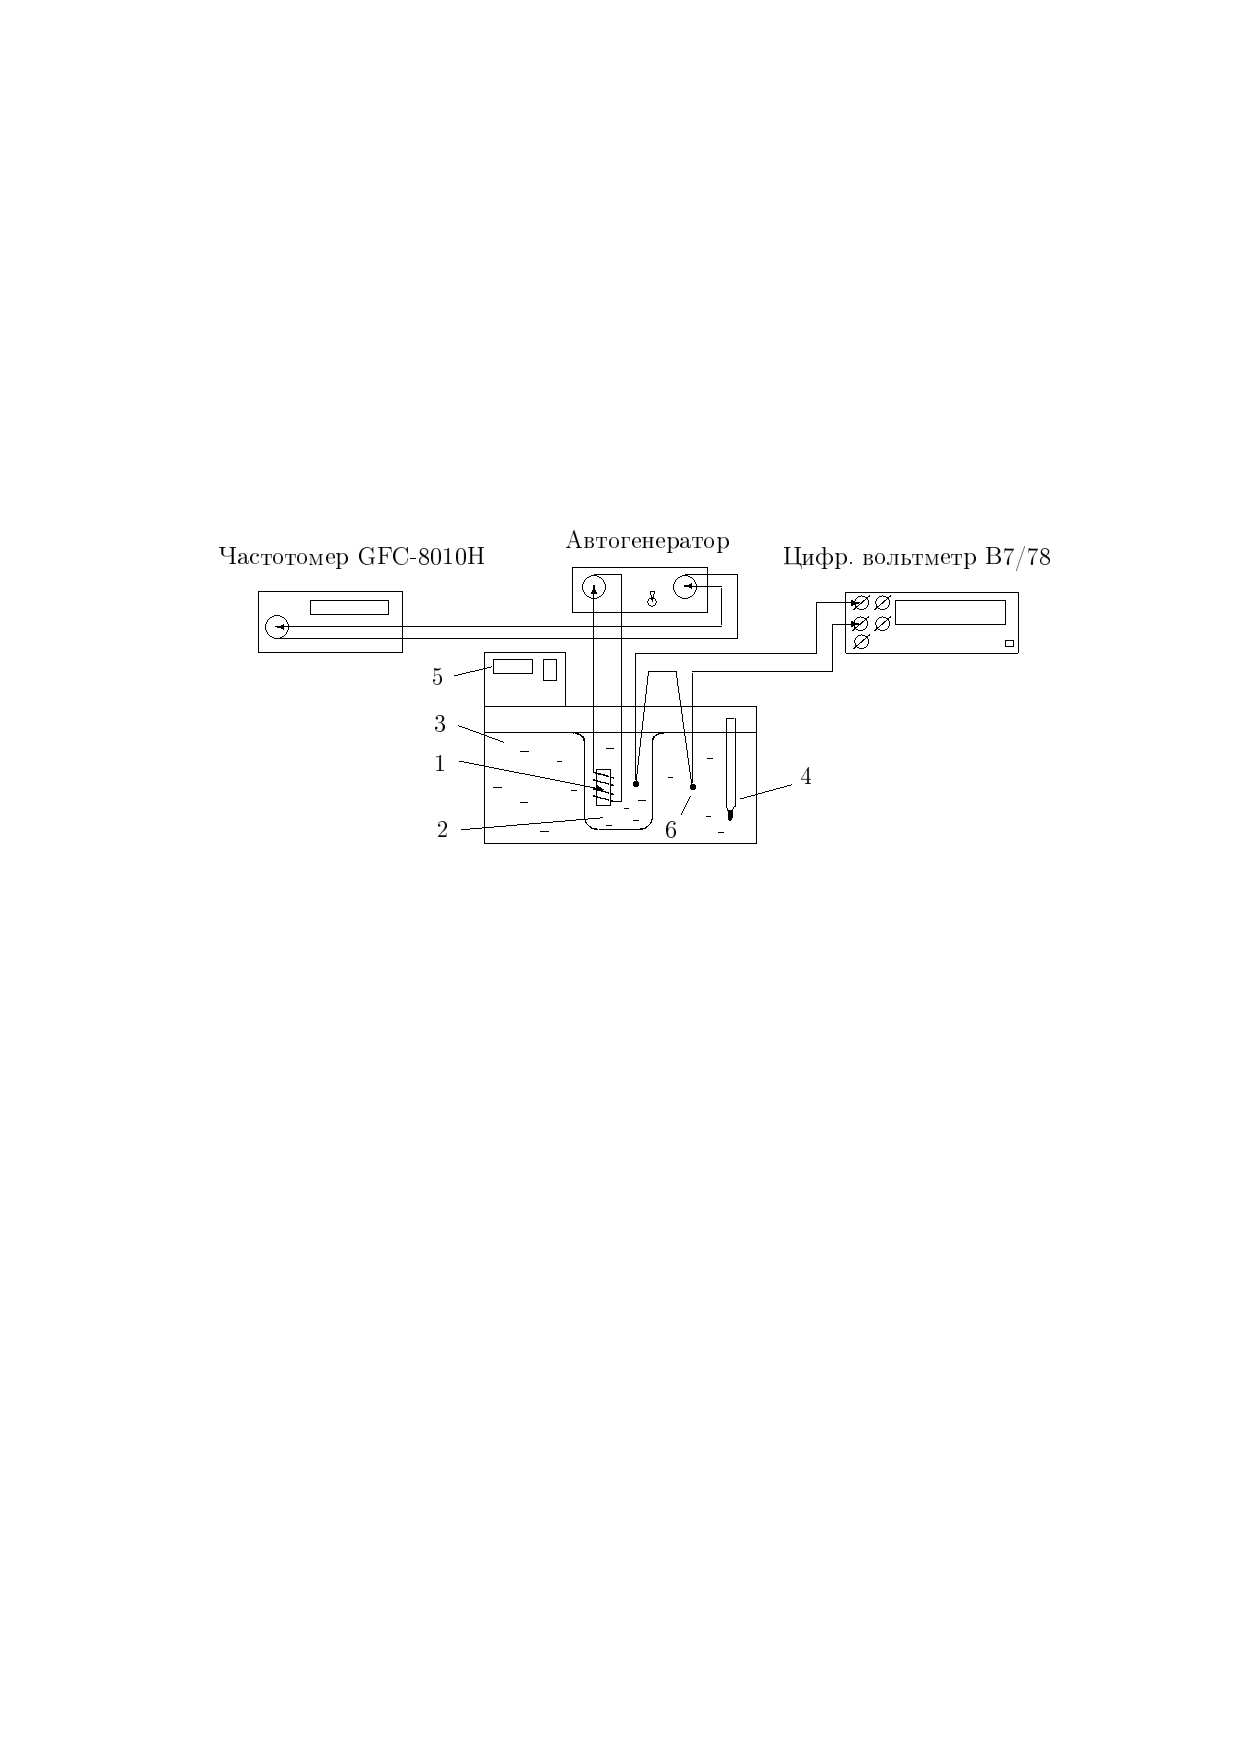
\includegraphics[scale=1]{ustanovka.pdf}}
		\caption{Схема экспериментальной установки.}
		\label{ris:ustanovka}
	\end{figure}
	
	Магнитная воосприимчивость образца $\chi$ определяется по изменению самоиндукции катушки. Обозначив через $L$ самоиндукцию катушки с образцом и через $L_0$ -- её самоиндукцию в отсутствие образца, получим
	\begin{equation*}
		(L-L_0)\propto \chi.
	\end{equation*}
	При изменении самоиндукции образца меняется период колебаний автогенератора:
	\begin{equation*}
		\tau = 2\pi \sqrt{LC},
	\end{equation*}
	где $C$ -- ёмкость конутра автогенератора. Период колебаний в отсуствие образца опредлеяется самоиндукцией пустой катушки:
	\begin{equation*}
		\tau_0 = 2\pi \sqrt{L_0C}.
	\end{equation*}
	Итак, закон Кюри-Вейсса справедлив, если выполнено соотношение:
	\begin{equation}
		\frac{1}{\chi} \propto (T-\Theta_p) \propto \frac{1}{\tau^2-\tau_0^2}
	\end{equation}
	
	%Измерения проводятся в интервале температур от 14$^\circ$C до 40$^\circ$C.

\section{Экспериментальные данные}
	

	\floatsetup[table]{capposition=top}	
	\begin{table}[H]
		\caption{Некоторые измеряемые величины и их погрешность.}
		\label{table:error}
		\begin{tabular}{|c|c|c|}
			\hline
			& $T$, $^\circ$C & $\tau$, мкс \\ \hline
			Величина          & 25,00          & 10,000      \\ \hline
			Погрешность       & 0,01           & 0,001       \\ \hline
			$\varepsilon$, \% & 0,04           & 0,01        \\ \hline
		\end{tabular}
	\end{table}

	\floatsetup[table]{capposition=top}	
	\begin{table}[H]
		\caption{Измеренные величины.}
		\label{table:results}
		\begin{tabular}{|c|c|c|c|c|}
			\hline
			$T$, $^\circ$C & $\tau$, мкс & $\mathscr{E}$, мкВ & $\Delta T,$ $^\circ$C & 1/($\tau^2$, - $\tau_0^2$), мкс$^{-2}$ \\ \hline
			12,1           & 10,873      & -10                & -0,24                 & 0,027                                  \\ \hline
			14,02          & 10,794      & -4                 & -0,10                 & 0,029                                  \\ \hline
			16,06          & 10,687      & -5                 & -0,12                 & 0,031                                  \\ \hline
			18,04          & 10,555      & -9                 & -0,22                 & 0,034                                  \\ \hline
			20,14          & 10,146      & -1                 & -0,02                 & 0,047                                  \\ \hline
			22,01          & 9,945       & -9                 & -0,22                 & 0,059                                  \\ \hline
			24,02          & 9,602       & -10                & -0,24                 & 0,096                                  \\ \hline
			26,05          & 9,428       & -9                 & -0,22                 & 0,141                                  \\ \hline
			28,04          & 9,344       & -9                 & -0,22                 & 0,182                                  \\ \hline
			30,07          & 9,287       & -7                 & -0,17                 & 0,225                                  \\ \hline
			32,04          & 9,256       & -10                & -0,24                 & 0,259                                  \\ \hline
			34,05          & 9,228       & -9                 & -0,22                 & 0,299                                  \\ \hline
			36,05          & 9,209       & -10                & -0,24                 & 0,334                                  \\ \hline
			38,05          & 9,194       & -10                & -0,24                 & 0,368                                  \\ \hline
			40,06          & 9,182       & -11                & -0,26                 & 0,400                                  \\ \hline
		\end{tabular}
	\end{table}

	Отметим, что чувствительность термопары составляет $k = 24$ $^\circ$C/мВ и период колбеаний пустой катушки есть $\tau_0 = 9,045$ мкс.
		
\newpage
\section {Обработка результатов}
	Построим график зависимости  $1/ (\tau^2 - \tau_0^2)$ от $T$ и МНК проведем прямую по точкам, расположенным в интервале от 21 до 41 $^\circ$C.
	\begin{figure}[H]
		\center{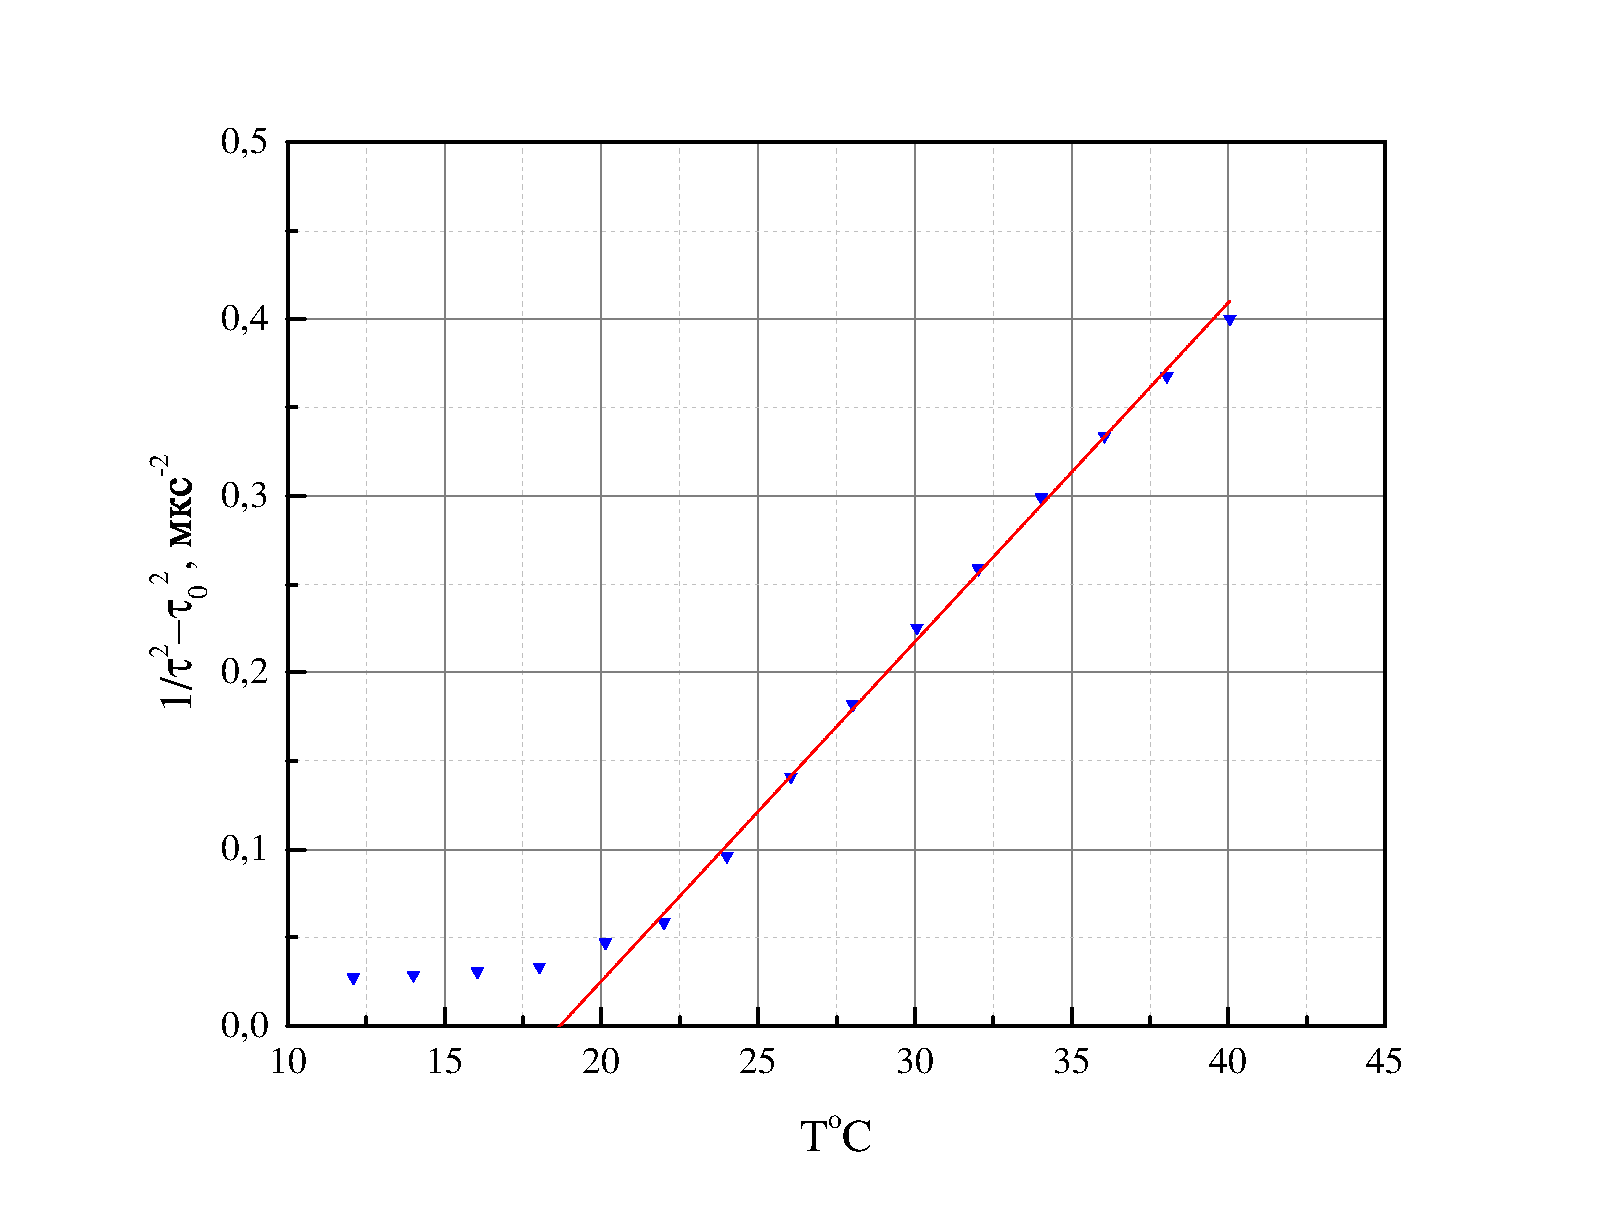
\includegraphics[scale=0.5]{graph.pdf}}
		\caption{Зависимость $1/ (\tau^2 - \tau_0^2)$ от $T$.}
		\label{ris:B=f(I)}
	\end{figure}

По графику определим температуру Кюри:
\[
	\boxed{\Theta_p = (18,7 \, \pm \, 0,3)^\circ \text{C}.}
\]
	
\section{Выводы}
	Определили температуру Кюри $\Theta_p = (18,7 \, \pm \, 0,3)^\circ \text{C}$, которая отличается от табличного значения 20,2 $^\circ$C на 7,4 \%.








\end{document}